\documentclass[Screen16to9,17pt]{foils}
\usepackage{zencurity-slides}

\usepackage{tabularx}
\usepackage{tikz}
\usetikzlibrary{mindmap,trees}
\usetikzlibrary{shapes.geometric, arrows,automata}
\usetikzlibrary{positioning}

\tikzset{
    state/.style={
           rectangle,
           rounded corners,
           draw=black, very thick,
           minimum height=2em,
           inner sep=2pt,
           text centered,
           },
}


% Email Security - domains, clients and servers

% This presentation will be focused on email security overall - from domains to clients to servers. The presentation will include a lot of acronyms and some technical details, the goal though is to get an overview of available technologies and their benefits.

% We will talk about domains and the current internet standards and recommendations for setting DNS records and features to optimise the reception of email securely - using encryption and certificates. Also which DNS records and features will prevent your domains from being abused for sending fake emails such as phishing with you as the sender.

% We will discuss client features which are considered dangerous, loading images automatically etc. and how to improve your client security by using only specific protocols with encryption.

% Servers will be discussed as examples of email architectures. Common blueprints for email will be discussed including which components are to be used for getting insights into your email security - reporting functions. Example open source software will be shown.

% The goal for this presentation is for participants to get an overview of current email security, to allow them to evaluate their own posture - and plan a strategy to improve email security, both personally and professionally.

% Keywords: SMTP, TLS, DNS MX, DNS TXT, DMARC, SPF, DKIM, SMTP DANE - RFC 7672, MTA Strict Transport Security (MTA-STS), SMTP TLS Reporting, OpenARC, DMARC reporting, Postfix, Dovecot, Lets Encrypt certificates and Open Source mail tools

% Note: This presentation will not cover much filtering of anti-virus, phishing and malware except recommend having incoming and outgoing proxy servers where such services can be provided.

% Slides will be in english, but presentation language danish.


% Måske medtage Tyklings email IP source tip!



\begin{document}
\selectlanguage{danish}
\mytitlepage{Email Security - domains, clients and servers}{2020}


\slide{Goal for today}

\hlkimage{5cm}{Shaking-hands_web.jpg}

This presentation will be focused on email security overall - from domains to clients to servers. The presentation will include a lot of acronyms and some technical details, the goal though is to get an overview of available technologies and their benefits.




\begin{list2}
\item Plan:
\item Approx 4h, with breaks
\item Inspiration for solving the tasks, prioritizing the tasks
\item I dont have tailer made solutions or easy answers for your organisation
\end{list2}

\slide{Todays Agenda - approximate time plan}

\begin{list2}
\item[\faClockO] 17:00 - 18:15 Part I: Client Security and Email Threats
\item 30min Break - eat, drink and socialize
\item[\faClockO] 18:45 - 19:30 Part II: Basic Email Services
\item 15min break
\item[\faClockO] 19:45 - 20:15 Part III: Testing Email Services
\item 15min break
\item[\faClockO] 20:30 - 21:00 Part IV: Strategy for Your Email Security
\end{list2}

Help me, thank you


\slide{Paranoia defined}

\hlkimage{12cm}{paranoia-definition.png}

Source: google paranoia definition


\slide{Hackers don't give a shit}

\hlkrightpic{11cm}{-3cm}{kiwicon-2009-hackers-dont-give-shit.jpg}

Your system is only for testing, development, ...

Your network is a research network, under construction, \\
being phased out, ...

Try something new, go to your management

Bring all the exceptions, all of them, update the risk \\
analysis figures - if this happens it is about 1mill DKK

Ask for permission to go full monty on your security

{\bf Think like attackers - don't hold back}


\slide{Confidentiality Integrity Availability}

\hlkimage{8cm}{cia-triad-uk.pdf}

\begin{list1}
\item We want to protect something
\item Confidentiality - data holdes hemmelige
\item Integrity - data ændres ikke uautoriseret
\item Availability - data og systemet er tilgængelige når de skal bruges
\end{list1}


\slide{Overlapping Security Incidents}

\hlkrightpic{12cm}{1cm}{datalaek-2019.png}

New data breaches nearly every week, these from danish news site \link{version2.dk}

Problem, we need to receive data from others

Data from others may contain malware

Have a job posting, yes\\
- then HR will be expecting CVs sent as .doc files



\slide{Email Security 2020}

\begin{list2}
\item DNS og email
\item TLS encryption settings
\end{list2}

\vskip 5mm
\centerline{Håber ikke I er alene om det, ellers vælg et par stykker ad gangen}



\slide{Part I: Client Security and Email Threats}

We will discuss client features which are considered dangerous, loading images automatically etc. and how to improve your client security by using only specific protocols with encryption.

\slide{The Internet Worm 2. nov 1988}

\begin{list1}
\item Exploited the following vulnerabilities
\begin{list2}
\item buffer overflow in fingerd - VAX code
\item Sendmail - DEBUG functionality
\item Trust between systems: rsh, rexec, ...
\item Bad passwords
\end{list2}
\item Contained camouflage!
\begin{list2}
\item Program name set to 'sh'
\item Used fork() to switch PID regularly
\item Password cracking using intern list of 432 words and /usr/dict/words
\item Found systems to infect in /etc/hosts.equiv, .rhosts, .forward, netstat ...
\end{list2}
\item Made byRobert T. Morris, Jr.
\end{list1}



\slide{Computer Viruses}

\begin{list1}
\item {\bf Definition 23-4} A \emph{computer virus} is a program that inserts (a possibly transformed version of) itself into one or more files and then performs some (possibly null) action.
\item Would spread through floppy disks and boot sector
\item Today more virus are spread through network shares, networked file systems
\begin{list2}
\item Boot sector virus - when booting a PC infects
\item A executable - exe files, similar types on PC platform .scr screensavers, .vbs visual basic scripts etc. Linux shell archives shar files.
\item Data - macro virus, found in Microsoft Office formats .doc etc.
\end{list2}
\item Polymorphic virus change their fingerprint/code during execution/infection
\end{list1}


\slide{Computer worms}

\begin{list1}
\item {\bf Definition 23-14} A \emph{computer worm} is a program that copies itself from one computer to another.
\item Computer worms has existed since research began mid-1970s
\item Morris Worm from November 2, 1988 was a famous example
\vskip 2cm
\item Virus, trojan or worm?\\
Unless you work specifically in the computer virus industry, call it all malware

\end{list1}



\slide{Trojan horses}

\begin{list1}
\item {\bf Definition 23-1} \emph{Malicious logic}, more commonly called \emph{malware}, is a set\\
 of instructions that cause a site's security policy to be violated.
\item {\bf Definition 23-2} A \emph{Trojan horse} is a program with an overt (documented or\\
known) purpose and a covert (undocumented or unexpected) purpose.

\item Lots of free applications on Android are in fact trojans

\item Book also mentions the Ken Thompson example with login program and compiler\\Insert Login backdoor, by inserting backdoor to notice when compiling compiler \smiley
\end{list1}

The history lesson
\url{https://en.wikipedia.org/wiki/Trojan_Horse}\\
\url{https://en.wikipedia.org/wiki/Trojan_horse_(computing)}

\slide{Ransomware}


\begin{list1}
\item {\bf Defition 23-21} \emph{Ransomware} is malware that inhibits the use of resources until a ransom usually monetary, is paid.
\item Book mentions 1989 example, PC CYBORG targetting PC/DOS computers
\item Uses cryptography to render data unreadable
\item Has become a huge problem for enterprises during the last 5-10 years
\item Often uses crypto-currencies today, like BitCoin (BTC) for payment
\item Often contains errors so decryption is impossible, or possible without payment!
\end{list1}


\slide{Phishing and spear phishing}


\begin{list1}
\item {\bf Definition 23-22} \emph{Phishing} is the act of impersonating a legitimate entity, typically a website associated with a business, in order to obtain information such as passwords, credit card numbers, and other private information without authorization
\item Example creating a fake bank website and make customers try to login
\item {\bf Definition 23-23} \emph{Spearphishing} is a phishing attack tailored for a particular victim.
\end{list1}


\slide{Malware defenses}


\begin{list1}
\item {\bf Theorem 23.2} It is undecidable whether an arbitrary program contains a malicious logic.
\item Scanning defenses,
\begin{list2}
\item Check disk and memory for known bad malware signatures
\item Check for changes - integrity protection
\end{list2}
\item Behavioural - what does a malware do, that normal programs dont
\item Static analysis - what does a program normally do, what does a malware do
\item Containment - change the environment to be more restricted
\end{list1}

\centerline{I dont trust or use anti-virus programs, fight me}

\slide{CVEs in popular mail programs}

\begin{list2}
\item
\end{list2}

\slide{Securing Thunderbird}

\begin{list2}
\item Security settings
\item Use TLS for SMTP
\item Use TLS for IMAPS
\item Disable loading of images
\item Disable sending version strings
\item Add plugins you need, but only those!
\end{list2}

Thunderbird mentioned as being one of the most popular email clients


\slide{Advanced: Run your mail client in a VM}

I run my email client in a VM, which can only connect to my mail server and my printer

\begin{alltt}\footnotesize
[hlk@dom0 ~]$ qvm-firewall Mailreader
NO  ACTION  HOST             PROTOCOL  PORT(S)  SPECIAL TARGET  ICMP TYPE  EXPIRE  COMMENT
0   accept  91.102.91.22/32  tcp       993      -               -          -       -
1   accept  91.102.91.22/32  tcp       587      -               -          -       -
2   accept  10.0.42.13/32    tcp       515      -               -          -       -
3   drop    -                -         -        -               -          -       -
[hlk@dom0 ~]$
\end{alltt}

\slide{Advanced: Removed last IP when sending through server}

Tykling blog example - hides the IP used when sending email, user privacy.

\slide{Part II: Basic Email Services}

We will talk about domains and the current internet standards and recommendations for setting DNS records and features to optimise the reception of email securely - using encryption and certificates. Also which DNS records and features will prevent your domains from being abused for sending fake emails such as phishing with you as the sender.

Servers will be discussed as examples of email architectures. Common blueprints for email will be discussed including which components are to be used for getting insights into your email security - reporting functions. Example open source software will be shown.

\slide{SMTP Simple Mail Transfer Protocol}

\begin{quote}
  The Simple Mail Transfer Protocol (SMTP) is a communication protocol for electronic mail transmission. As an Internet standard, SMTP was first defined in 1982 by RFC 821, and updated in 2008 by RFC 5321 to Extended SMTP additions, which is the protocol variety in widespread use today. Mail servers and other message transfer agents use SMTP to send and receive mail messages.
\end{quote}

\url{https://en.wikipedia.org/wiki/Simple_Mail_Transfer_Protocol}


\slide{SMTP Simple Mail Transfer Protocol}

\begin{alltt}\tiny
hlk@bigfoot:hlk$ telnet mail.kramse.dk 25
Connected to sunny.
220 sunny.kramse.dk ESMTP Postfix
HELO bigfoot
250 sunny.kramse.dk
MAIL FROM: Henrik
250 Ok
RCPT TO: hlk@kramse.dk
250 Ok
DATA
354 End data with <CR><LF>.<CR><LF>
hejsa
.
250 Ok: queued as 749193BD2
QUIT
221 Bye
\end{alltt}

\begin{list2}
\item RFC-821 SMTP Simple Mail Transfer Protocol fra 1982
\item \link{http://en.wikipedia.org/wiki/Simple_Mail_Transfer_Protocol}
\end{list2}



\slide{Email Software}

My recommendations are:
\begin{list2}
\item Sending mail with SMTP using Postfix
\item Receiving mail with IMAP using Dovecot
\end{list2}

I would NOT use these:
\begin{list2}
\item Exim - multiple Remote Code Execution in 2019, fatal security vulns \\
\url{https://www.exim.org/static/doc/security/}
\item OpenSMTPD has had some really strange vulnerabilities recently\\
\url{https://www.opensmtpd.org/security.html}
\item Dont use Sendmail - old and horrible
\end{list2}


Dont use , Dont use OpenSMTPD


\slide{Example of SMTP and IMAP}

\begin{center}
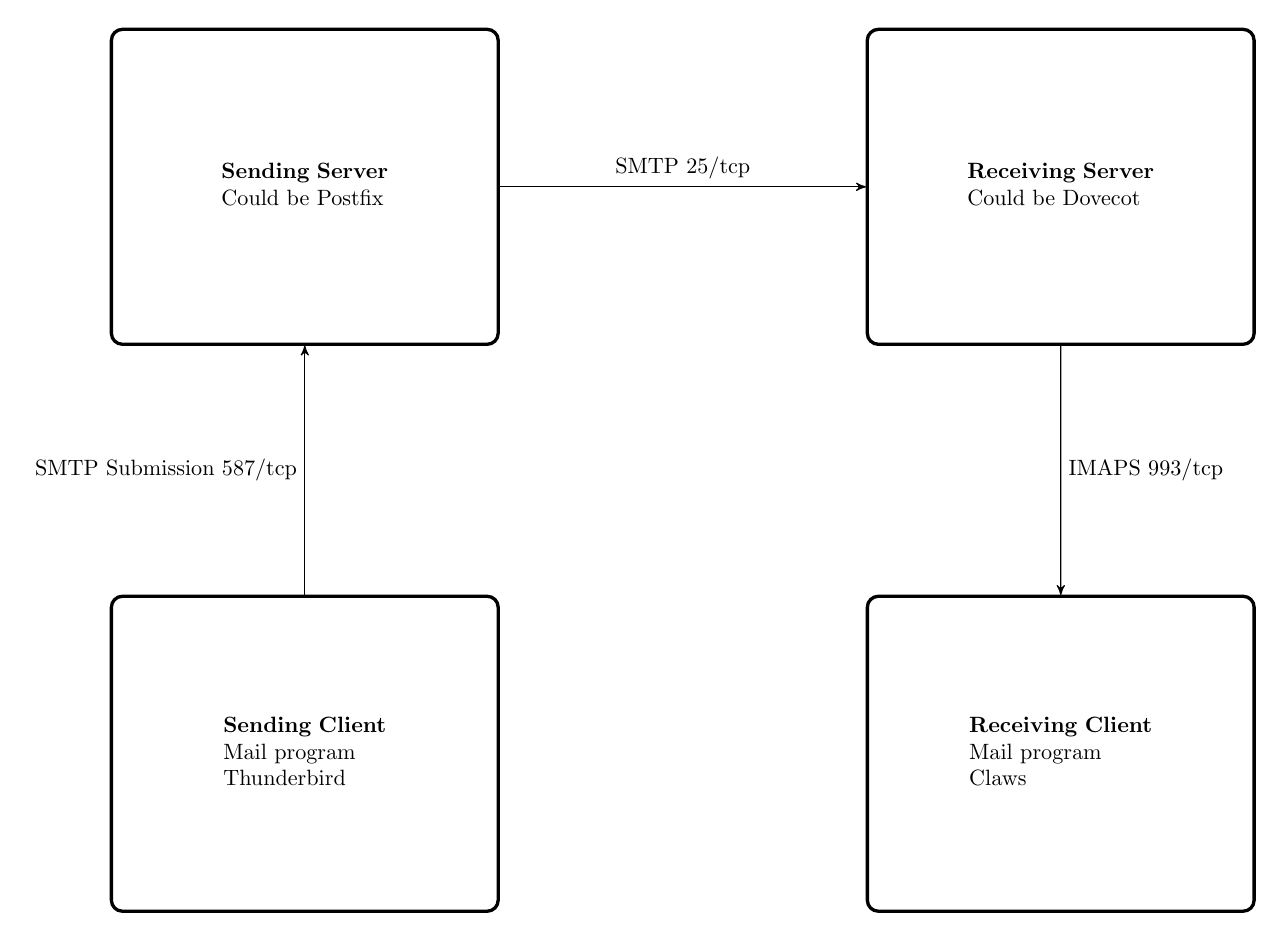
\begin{tikzpicture}[->,>=stealth',scale=0.8, transform shape]
  \newlength{\boxwidth}
  \setlength{\boxwidth}{6cm}
  \newlength{\boxheight}
  \setlength{\boxheight}{5cm}
  \newlength{\boxspace}
  \setlength{\boxspace}{12cm}

  % http://texample.net/tikz/examples/epc-flow-charts/

  % https://www.overleaf.com/learn/latex/LaTeX_Graphics_using_TikZ:_A_Tutorial_for_Beginners_(Part_3)%E2%80%94Creating_Flowcharts

   % Use previously defined 'state' as layout (see above)
   % use tabular for content to get columns/rows
   % parbox to limit width of the listing
   \node[state,text width=\boxwidth,minimum height=\boxheight] (SENDER)
   {\begin{tabular}{l}
   {\bf Sending Server}\\
      Could be Postfix
   \end{tabular}};

   %
   \node[state,         % layout (defined above)
    text width=\boxwidth,       % max text width
    minimum height=\boxheight,
    %yshift=2cm,                % move 2cm in y
    right of=SENDER,    % Position is to the right of QUERY
    node distance=\boxspace,    % distance to First node
    anchor=center] (RECEIVER)   % posistion relative to the center of the 'box'
   {%
   \begin{tabular}{l}
   {\bf Receiving Server}\\
Could be Dovecot
   \end{tabular}};

   \node[state,
    below of=SENDER,
    yshift=-8cm,
    anchor=center,
    minimum height=\boxheight,
    text width=\boxwidth] (THUNDERBIRD)
   {%
   \begin{tabular}{l}
   {\bf Sending Client}\\
    Mail program\\
    Thunderbird
   \end{tabular}
   };

   \node[state,
    below of=RECEIVER,
    yshift=-8cm,
    anchor=center,
    minimum height=\boxheight,
    text width=\boxwidth] (CLAWS)
   {%
   \begin{tabular}{l}
   {\bf Receiving Client}\\
    Mail program\\
    Claws
   \end{tabular}
   };
   % draw the paths and and print some Text below/above the graph
   \path
   (SENDER)     edge node[anchor=north,above]{SMTP 25/tcp} (RECEIVER)
   (THUNDERBIRD)        edge node[anchor=west,left]{SMTP Submission 587/tcp} (SENDER)
   (RECEIVER) edge node[anchor=east,right]{IMAPS 993/tcp }   (CLAWS);

\end{tikzpicture}
\end{center}



\slide{Postfix}

\hlkimage{3cm}{postfix-mouse.png}

\begin{quote}
  Postfix is a free and open-source mail transfer agent (MTA) that routes and delivers electronic mail.

It is released under the IBM Public License 1.0 which is a free software license. Alternatively, starting with version 3.2.5, it is available under the Eclipse Public License 2.0 at the user's option.[2]

Originally written in 1997 by Wietse Venema at the IBM Thomas J. Watson Research Center in New York, and first released in December 1998[3], Postfix continues as of 2020 to be actively developed by its creator and other contributors.
\end{quote}
Source: \url{https://en.wikipedia.org/wiki/Postfix_(software)}

Home page: \url{http://www.postfix.org/}


\slide{Dovecot}

\begin{quote}
Dovecot is an open-source IMAP and POP3 server for Unix-like operating systems, written primarily with security in mind.[3] Timo Sirainen originated Dovecot and first released it in July 2002. Dovecot developers primarily aim to produce a lightweight, fast and easy-to-set-up open-source email server.

The primary purpose of Dovecot is to act as mail storage server. Mail is delivered to the server using some mail delivery agent (MDA) and stored for later access with an email client (mail user agent, or MUA).
\end{quote}
Source: \url{https://en.wikipedia.org/wiki/Dovecot_(software)}

\begin{quote}
Dovecot is an open source IMAP and POP3 email server for Linux/UNIX-like systems, written with security primarily in mind. Dovecot is an excellent choice for both small and large installations. It's fast, simple to set up, requires no special administration and it uses very little memory.
\end{quote}
Home page: \url{https://www.dovecot.org/}




\slide{Attacking Email }


\slide{Fokus: DNS og email}

\hlkrightpic{10cm}{-2cm}{brian-patrick-tagalog-680954-unsplash.jpg}
{~}

\begin{list2}
\item Vi er afhængige af email, modtagelse og afsendelse
\item Når vi modtager skal det helst gå hurtigt
\item Når vi sender skal vi ikke ende i spam mappen
\item Phishing, hvem kan sende \emph{fra vores domæne}
\end{list2}


\slide{Various key attack types, clients and employees}

\begin{list2}
\item Phishing - sending fake emails, to collect credentials
\item Spear phishing - targetted attacks
\item Person in the middle - sniffing and changing data in transit
\item Drive-by attacks - web pages infected with malware, often ad servers
\item Malware transferred via USB or email
\item Credential Stuffing, Password related, like re-use of password, see slide about being pwned
\end{list2}

\vskip 1cm
\centerline{\Large\bf If we all wait a bit, and not click links immediately}

\vskip 1cm
Hackers try to create "urgency", click this or loose money




\slide{Internet i dag}

\hlkimage{10cm}{images/server-client.pdf}

\begin{list1}
\item Klienter og servere
\item Rødder i akademiske miljøer
\item Protokoller der er op til 20 år gamle
\item Meget lidt kryptering, mest på http til brug ved e-handel
\end{list1}



\slide{Data found in Network traffic }

\begin{list1}
\item Many older internet protocols are cleartext - no encryption
\item Lets take an example, DNS
\item Domain Name System DNS breadcrumbs
\begin{list2}
\item Your company domain, mail servers
\item Emails being sent are essentially post cards
\end{list2}
\vskip 1cm
\item Advice show your users, ask them to participate in a experiment
\item Sniffing a wireless network is easy
\end{list1}

\vskip 2 cm
\centerline{\bf\Large Maybe use VPN more - or always!}




\slide{DNS er mere end navneopslag}

% DNS MX, DNS TXT

\begin{list1}
  \item består af resource records med en type:
    \begin{list2}
\item adresser A-records
\item IPv6 adresser AAAA-records
\item autoritative navneservere NS-records
\item post, mail-exchanger MX-records
\item flere andre: md ,  mf ,  cname ,  soa ,
                  mb , mg ,  mr ,  null ,  wks ,  ptr ,
                  hinfo ,  minfo ,  mx ....
\end{list2}
\end{list1}
\begin{alltt}
        IN      MX      10      mail.zencurity.dk.
        IN      MX      20      mail2.zencurity.dk.
\end{alltt}





\slide{DNSSEC get started now}

\hlkimage{12cm}{cz-nic-dnssec-tlsa-validator.png}

\begin{quote}
"TLSA records store hashes of remote server TLS/SSL certificates. The authenticity of a TLS/SSL certificate for a domain name is verified by DANE protocol (RFC 6698). DNSSEC and TLSA validation results are displayer by using several icons."
\end{quote}


\slide{Crypto slides here!?}

\slide{SSL og TLS}

\hlkimage{5cm}{crypto-class.png}

\begin{list1}
\item Oprindeligt udviklet af Netscape Communications Inc.
\item Secure Sockets Layer SSL er idag blevet adopteret af IETF og kaldes
derfor også for Transport Layer Security TLS
TLS er baseret på SSL Version 3.0
\item RFC-2246 The TLS Protocol Version 1.0 fra Januar 1999
\item RFC-3207 SMTP STARTTLS
\item Det er svært!
\item Stanford Dan Boneh udgiver en masse omkring crypto\\ \link{https://crypto.stanford.edu/~dabo/cryptobook/}
\end{list1}





\slide{Fokus: Encryption and TLS settings}

%\hlkimage{16cm}{bettercrypto-nginx.png}

\begin{list2}
\item Check your TLS settings multiple times a year
\item Easy for web servers Qualys sslscan
\item Almost as easy with a command line tool
\end{list2}


\slide{DNSSEC and DANE}

\begin{quote}
"Objective:

Specify mechanisms and techniques that allow Internet applications to
establish cryptographically secured communications by using information
distributed through DNSSEC for discovering and authenticating public
keys which are associated with a service located at a domain name."
\end{quote}

\begin{list1}
\item DNS-based Authentication of Named Entities (dane)
\end{list1}


\slide{Part III: Testing email services}

\slide{Hackertools are for everyone!}

\hlkimage{2cm}{hackers_JOLIE+1995.jpg}


\begin{list2}
\item Hackers work all the time to break stuff, Use hackertools:
\item Nmap, Nping \link{http://nmap.org}
\item Wireshark - \link{http://www.wireshark.org/}
\item Aircrack-ng \link{http://www.aircrack-ng.org/}
\item Kali Linux \link{http://www.kali.org}
\end{list2}

\vskip 5mm
\centerline{Most popular hacker tools \link{http://sectools.org/}}

\slide{Nmap the world}

\hlkimage{19cm}{trinity-nmapscreen-hd-cropscale-418x250.jpg}

\slide{Really do Nmap your world}

\hlkimage{8cm}{nmap-zenmap.png}

\begin{list2}
\item Nmap is a port scanner, but does more
\item Finding your own infrastructure available from the guest network?
\item See your printers having all the protocols enabled AND a wireless?
\end{list2}

\slide{Generic Encryption settings sslscan}

\begin{list2}
\item Easy to use tool \verb+sslscan www.domain.tld+
\item Check TLS/SSL on Web Servers
\item Check TLS/SSL on other services -- Mail servers
\end{list2}

\slide{Hacking is not magic}

\hlkimage{11cm}{ninjas.png}

\begin{list2}
\item Hacking only requires some ninja training
\item We have been doing this since 1995 when SATAN was released
\item Listen, Plan, Act, Do hacking
\end{list2}

\slide{Book: Linux Basics for Hackers (LBfH)}

\hlkimage{4cm}{LinuxBasicsforHackers_cover-front.png}

\emph{Linux Basics for Hackers
Getting Started with Networking, Scripting, and Security in Kali}
by OccupyTheWeb
December 2018, 248 pp.
ISBN-13:
9781593278557

\link{https://nostarch.com/linuxbasicsforhackers}

\slide{Book: Kali Linux Revealed (KLR)}

\hlkimage{6cm}{kali-linux-revealed.jpg}

\emph{Kali Linux Revealed  Mastering the Penetration Testing Distribution}

\link{https://www.kali.org/download-kali-linux-revealed-book/}\\
explains how to install Kali Linux




\slide{Nmap efter SSL og TLS}

\hlkimage{7cm}{nmap-sslv2.png}

\begin{list1}
\item Nu vi har lært Kali og Nmap at kende
\begin{list2}
\item Find nemt alle ssl version 2 og 3\\
\verb+nmap --script ssl-enum-ciphers+
\item Brug ssllabs https://www.ssllabs.com/
\end{list2}
\end{list1}


\slide{sslscan}

\begin{alltt}\small
root@kali:~# sslscan --ssl2 web.kramse.dk
Version: 1.10.5-static
OpenSSL 1.0.2e-dev xx XXX xxxx

Testing SSL server web.kramse.dk on port 443
...
  SSL Certificate:
Signature Algorithm: sha256WithRSAEncryption
RSA Key Strength:    2048

Subject:  *.kramse.dk
Altnames: DNS:*.kramse.dk, DNS:kramse.dk
Issuer:   AlphaSSL CA - SHA256 - G2
\end{alltt}

Source:
Originally sslscan from http://www.titania.co.uk
 but use the version on Kali

SSLscan can check your own sites, while Qualys SSLLabs only can test from hostname


\slide{Part IV: Strategy for Your Email Security}

The goal for this presentation is for participants to get an overview of current email security, to allow them to evaluate their own posture - and plan a strategy to improve email security, both personally and professionally.

Make sure everyone attending know about methods to restrict sending of false
emails, how to secure this using DNSSEC, SPF, DMARC - DNS based updates to your
email domain security



\slide{Email security -- Goals}

\begin{list2}
\item SPF Sender Policy Framework\\ {\footnotesize\link{https://en.wikipedia.org/wiki/Sender_Policy_Framework}}
\item DKIM DomainKeys Identified Mail\\
{\footnotesize\link{https://en.wikipedia.org/wiki/DomainKeys_Identified_Mail}}
\item DMARC Domain-based Message Authentication, Reporting and Conformance\\
{\footnotesize\link{https://en.wikipedia.org/wiki/DMARC}}
\item DANE DNS-based Authentication of Named Entities\\ {\footnotesize\link{https://en.wikipedia.org/wiki/DNS-based_Authentication_of_Named_Entities}}
\item Brug allesammen, check efter ændringer!
\end{list2}

\centerline{Jeg er glad for at teste med \link{https://dmarcian.com/}}


\slide{SPF}

 SPF Sender Policy Framework\\ {\footnotesize\link{https://en.wikipedia.org/wiki/Sender_Policy_Framework}}


\slide{DKIM}

 DKIM DomainKeys Identified Mail\\
 {\footnotesize\link{https://en.wikipedia.org/wiki/DomainKeys_Identified_Mail}}



\slide{DMARC}
%

DMARC Domain-based Message Authentication, Reporting and Conformance\\
{\footnotesize\link{https://en.wikipedia.org/wiki/DMARC}}


\slide{DMARC for non-sending Domains}
If you have domains that \emph{never send email} then add the following SPF and DMARC to avoid misuse.

from my own DSN template for \emph{parked domains}:
\begin{alltt}
gdns.template   v=spf1 -all     43200
_dmarc.gdns.template    v=DMARC1; p=reject;     43200
\end{alltt}


\slide{DANE}
 DANE DNS-based Authentication of Named Entities\\ {\footnotesize\link{https://en.wikipedia.org/wiki/DNS-based_Authentication_of_Named_Entities}}

SMTP DANE - RFC 7672,

\slide{MTA-STS}

MTA Strict Transport Security (MTA-STS)

\slide{Authenticated Received Chain (ARC)}
RFC 8617
The Authenticated Received Chain (ARC) Protocol, JULY 2019

https://www.rfc-editor.org/info/rfc8617
OpenARC

\slide{Get Started and Get Resources}

{\bf Suggested method:}\\
Use services on the internet, such as \link{https://internet.nl/} and \link{https://dmarcian.com/} to see current status for your domains.

{\bf Hints:}\\
I suggest the following strategy when you implement these methods, if you dare do it right now. If you make a plan.

{\bf Basic mail security 2019}
\begin{enumerate}
\item Implement DNSSEC - turn it on, most likely easy
\item Configure Sender Policy Framework, perhaps only \verb+~all+ tilde means soft fail
\item Configure DomainKeys Identified Mail
\item Configure receiving email address for DMARC
\item Configure Domain-based Message Authentication - reject none
\end{enumerate}


{\bf Advanced mail security 2019}
\begin{enumerate}
\item Create real certificates for TLS and DANE, I use Lets Encrypt
\item Publish them \smiley
\end{enumerate}

Take domain(s) of your choice and make a table:

\begin{tabularx}{\textwidth}{|X|l|l|l|l|l|l|} \hline
Domain \faEnvelopeO & DNS NS 2+ & DNSSEC & SPF & DKIM & DMARC & DANE \\\hline
zencurity.com & \faCheck & \faCheck & \faCheck &  & \faCheck & \\ \hline

 &  &  &  & & & \\\hline
 &  &  &  & & & \\\hline
\end{tabularx}

{\bf Discussion:}\\
You need to research before making changes to important domains.




\slide{Graphs and Dashboards!}

\hlkimage{10cm}{illustrated-screenshot-hero-kibana.png}

Screenshot from \url{https://www.elastic.co/kibana}

{\bf Suggested method:}\\
Visit the web page for \emph{Getting started with the Elastic Stack} :\\
{\footnotesize\url{https://www.elastic.co/guide/en/elastic-stack-get-started/current/get-started-elastic-stack.html}}


\slide{Email tools are abundant}

%\hlkimage{14cm}{Logstash1.png}
Spend some time trying different tools for DMARC reporting. A month or a week, depending on the domain and your users. Github alone has 100s of projects concerned with parsing, reporting and working with DMARC.

Then after some time has passed, and you have reviewed reporting from DMARC, turn it on for real:
\begin{enumerate}
\item Configure SPF to disallow with hard fail use \verb+-all+ minus
\item Configure DMARC with reject - reject emails not following policy
\end{enumerate}


\begin{list2}
\item Before implementing security, monitor your services
\item DMARC Analysis and reporting tools
\item SMTP TLS Reporting
\end{list2}


\slide{Scripts for doing Lets Encrypt mail certificate}

Lets Encrypt certificates
input Sunny configurations

\slide{Advanced Network tools - examples}

\hlkimage{12cm}{kibana-solido.png}

\begin{list2}
\item Net: Bro \link{http://www.bro-ids.org} Suricata \link{http://suricata-ids.org}
\item DNS: DSC and PacketQ \link{https://github.com/dotse/packetq/wiki}
\item Syslog: Elasticsearch, Logstash, and Kibana, called ELK stack or Elastic stack
\item Use these to see inside systems using DNS and SMTP for unauthorized traffic
\end{list2}


\slide{Storing query logs, old school or needed?}

\hlkimage{6cm}{bro-sample-ssl-scripts.png}

\begin{list2}
\item DNS query logs, keep it for at least a week?\\
- with DSC and PacketQ \link{https://github.com/DNS-OARC/PacketQ}
\item SSL/TLS log with Bro/Suricata\\
{\footnotesize\link{https://www.bro.org/sphinx-git/script-reference/scripts.html}}
\item Log with Elasticsearch?\\
{\footnotesize\link{https://www.elastic.co/guide/en/elasticsearch/guide/current/index.html}}
%\item Even netflow session logging, full 1:1 - NFSen, Suricata Flow mode?
%\item Moloch \link{https://github.com/aol/moloch}
\end{list2}

\centerline{Uetisk? eller smart hvis man vil spore hvor malware kom ind}



\myquestionspage

\slide{Extras}

\slide{Book: Defensive Security Handbook (DSH)}

\hlkimage{6cm}{defensive-security-handbook.jpg}

\emph{Defensive Security Handbook: Best Practices for Securing Infrastructure}, Lee Brotherston, Amanda Berlin ISBN: 978-1-491-96038-7

\slide{Reading List}

\begin{list1}
\item Read ATT\&CK 101 Blog Post\\
\link{https://medium.com/mitre-attack/att-ck-101-17074d3bc62}
\item and browse MITRE ATT\&CK web site\\ \link{https://attack.mitre.org/}
\end{list1}


\slide{Hardenize - web sites with testing}

\begin{list1}
\item Multiple sites provide testing of domains and configurations
\item \link{https://www.hardenize.com/}
\item \link{https://internet.nl/}
\item \link{https://observatory.mozilla.org/} - try www.zencurity.dk which fails
\item \link{https://www.ssllabs.com/}
\item \link{https://securityheaders.com/}
\item \link{https://webbkoll.dataskydd.net/en}
\item Using the available protocols can make your \emph{cookies} better protected, use the \emph{secure} and \emph{http only} along with HSTS, strict transport etc.
\end{list1}

Now we will check our own sites, and create plans. Which parts are most interesting to you? Not having your domains abused for spamming or headers and security of your own web sites?




\end{document}
